\newpage
\clearpage
\section{Detector setup}
    \subsection{Large Hadron Collider}
        The Large Hadron Collider (LHC) is the world's largest circular accelerator. Figure \ref{LHC} shows that the LHC and its major experimental collaborations are located near Geneva, Switzerland. LHC Run 1 was conducted from 2009 to 2013, and Run 2 followed from 2015 to 2018.\@ The ongoing Run 3 is scheduled to collect physics data from 2022 to the summer of 2026.\@ During this period, most measurements focus on proton-proton collisions, with heavy-ion collision measurements conducted for about one month each year. The LHC hosts four major experimental collaborations: ATLAS, CMS, LHCb, and ALICE.\@
        \begin{figure}[htbp]
            \centering
            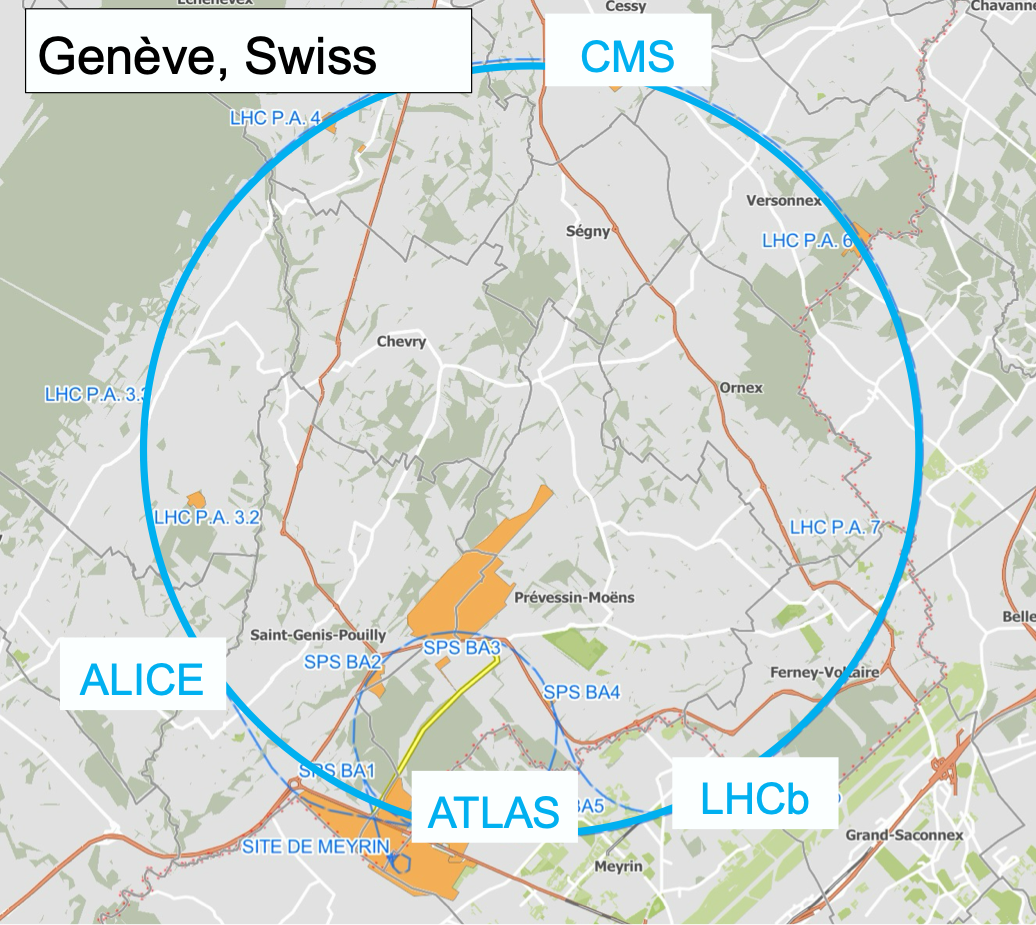
\includegraphics[keepaspectratio, scale=0.2]{fig/2_1_LHC_detecter.png}
            \caption{LHC}
            \label{LHC}
        \end{figure}
        \subsection{A Large Ion Collider Experiment}
        The A Large Ion Collider Experiment (ALICE) collaboration is an international effort of 168 research institutions from 40 countries and approximately 2,000 researchers. The overall view of the ALICE detector is shown in Figure \ref{ALICE_detectors}. The ALICE detector system is dedicated to studying the Quark-Gluon Plasma (QGP) produced in heavy-ion collisions.
        \begin{figure}[htbp]
            \centering
            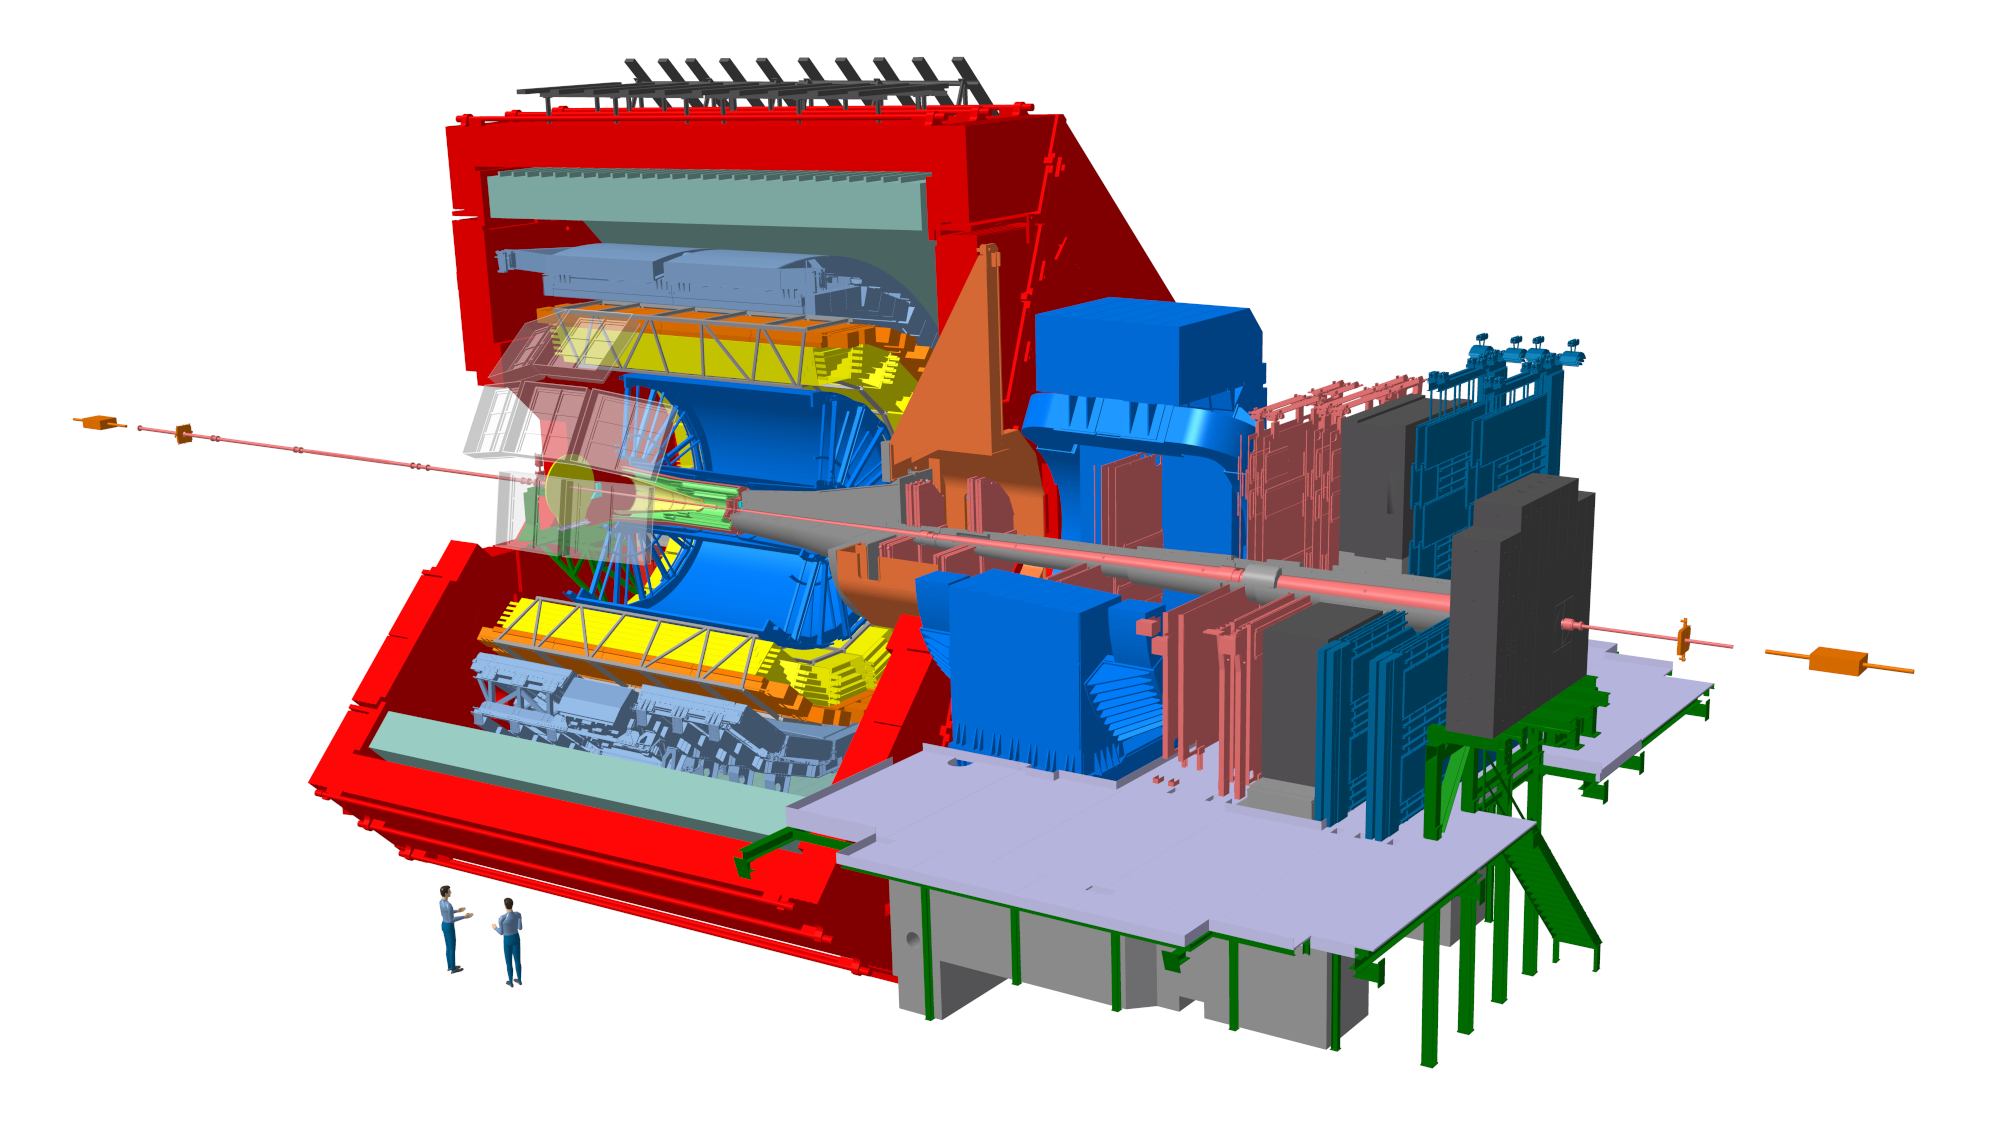
\includegraphics[keepaspectratio, scale=0.2]{fig/2_1_ALICE_RUN3_detectors.jpg}
            \caption{ALICE detectors}
            \label{ALICE_detectors}
        \end{figure}
        The detectors can be broadly divided into two main groups: the barrel detectors and the forward detectors.
        The barrel detectors include ITS, TPC, TOF, EMCal, TRD, PHOS/CPV, and HMPID detectors.\@ A magnetic field is applied along the beam axis, bending the motion of charged particles and enabling particle identification, momentum, and energy measurements. The forward detectors are specifically designed for muon measurements and consist of three trackers—MFT, MCH, and MID—and two hadron absorbers. A dipole magnet is placed between MCH, allowing the measurement of muon momentum and sign. Other detectors include the ZDC and FIT.\@ The ZDC is located far from the collision point and measures the number of neutrons and protons, determining the centrality of heavy-ion collision events. The FIT detectors are located forward and backward near the collision point to measure the event luminosity and particle multiplicity.
        \subsubsection{MUON Spectrometer}
            \begin{figure}
                \centering
                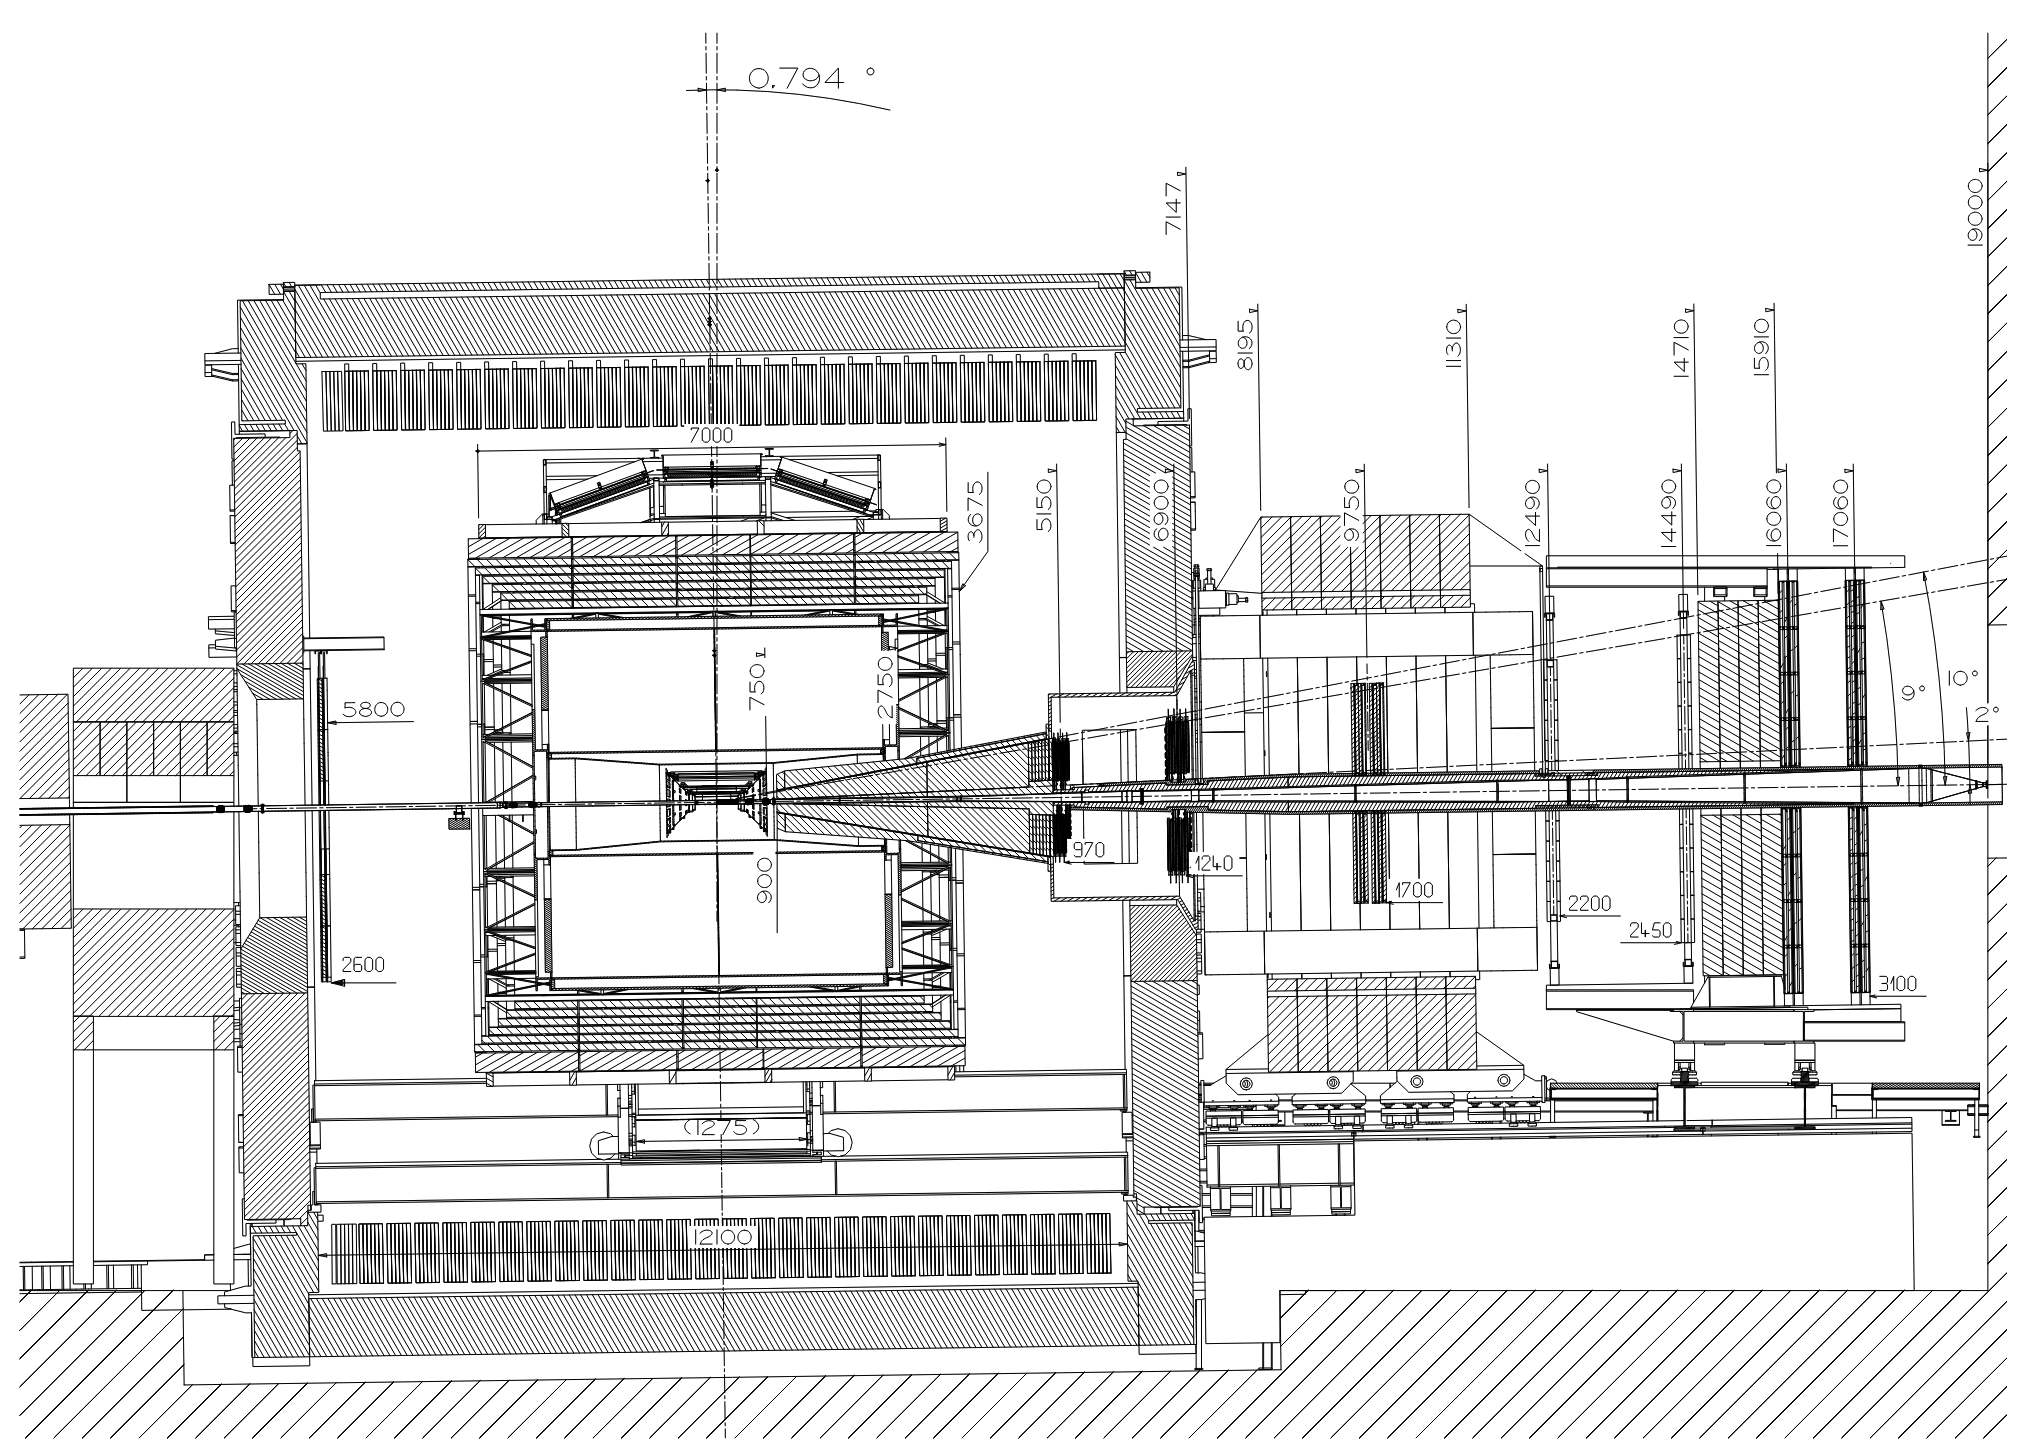
\includegraphics[keepaspectratio, scale=0.25]{fig/2_2_MUONspectrometer.png}
                \caption{MUON spectrometer}
                \label{MUONspectrometer}
            \end{figure}
            The MUON spectrometer is shown in Figure \ref{MUONspectrometer}\cite{Muon_TDR}. The MUON spectrometer consists of the Front Absorber, MCH, Iron Wall, and MID with an acceptance range of $-4.0 < \eta < -2.5$. It utilizes the high penetration power of muons for their identification. Various particles generated at the collision point (IP) pass through the Front Absorber. Hadrons and light electrons, which interact strongly, are absorbed by the Front Absorber, while the muons, due to their high penetration power, pass through it. The muons that pass through the Front Absorber are detected, and any particles such as $\pi$ mesons produced from interactions within the Front Absorber are measured by the MCH.\@ These particles are absorbed in the Iron Wall, preventing the MID from detecting them.\@ Therefore, muon identification is performed by combining tracks measured in the MCH and MID.\@ The momentum of the muons is measured using a dipole magnet in the MCH, which is set to a magnetic flux density of 3.0 $\mathrm{T/m^2}$.\@
        \subsubsection{MFT}
            \begin{figure}[htbp]
                \centering
                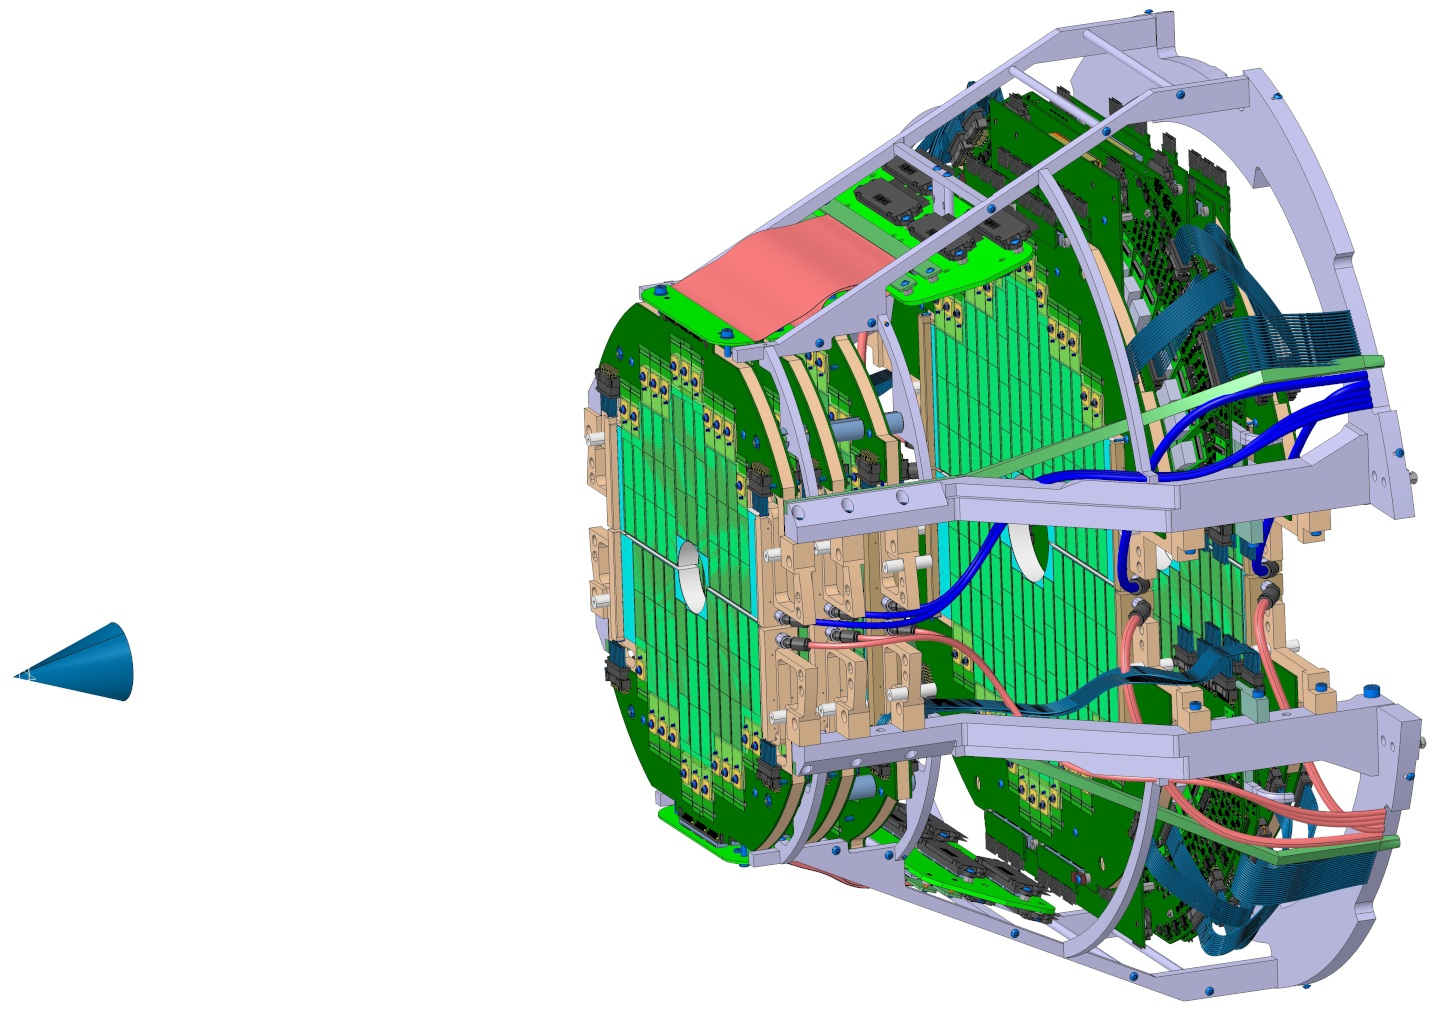
\includegraphics[keepaspectratio, scale=0.17]{fig/2_3_MFT.jpg}
                \caption{MFT}
                \label{MFT}
            \end{figure}
            The MUON spectrometer is shown in Figure \ref{MFT}\cite{MFT_TDR}. The MFT is a newly installed silicon pixel detector positioned between $z = -46.0$ and $z = -76.8$ cm, with an acceptance range of $-3.6 < \eta < -2.5$ in Run 3. It consists of five layers of disks that detect tracks and reconstructs standalone MFT tracks, taking into account the influence of the L3 magnet, which generates the ALICE central magnetic field. Since the detector is placed in front of the Front Absorber, the measured tracks include muons as well as various other particles, such as $\pi$ mesons and $K$ mesons. By combining these tracks with those measured by the backward MUON spectrometer, the $DCA$ of the muons can be determined. This capability allows for the separation of muons originating from $c$ and $b$ quarks, based on lifetime differences. Additionally, the precision of the opening angle between the muon pair is improved, enhancing mass resolution. Furthermore, since the MFT is positioned in front of the Front Absorber, it allows for the measurement of muons with lower transverse momentum compared to those measured by the MUON spectrometer alone.

        \subsubsection{MFT-MUON Track Matching}\label{MFT-MUON_matching}
            The Global Track was reconstructed using the MCH track measured by the MUON spectrometer and the MFT track measured by the MFT detector. First, the MCH tracks measured by the MUON spectrometer are extrapolated toward the collision point, extending up to the last disk of the MFT, located at $z = 76.8$ cm. This extrapolation accounts for multiple scattering and energy loss corrections in the Front Absorber, which is located between the MUON spectrometer and the MFT. Next, suitable MFT tracks are selected based on both their position and direction, and the matching quality is evaluated by comparing the position and slope of the tracks. The MFT track with the best matching quality is selected and used to construct the Global Track.
            %begin{figure}[htbp]
            %    \centering
            %    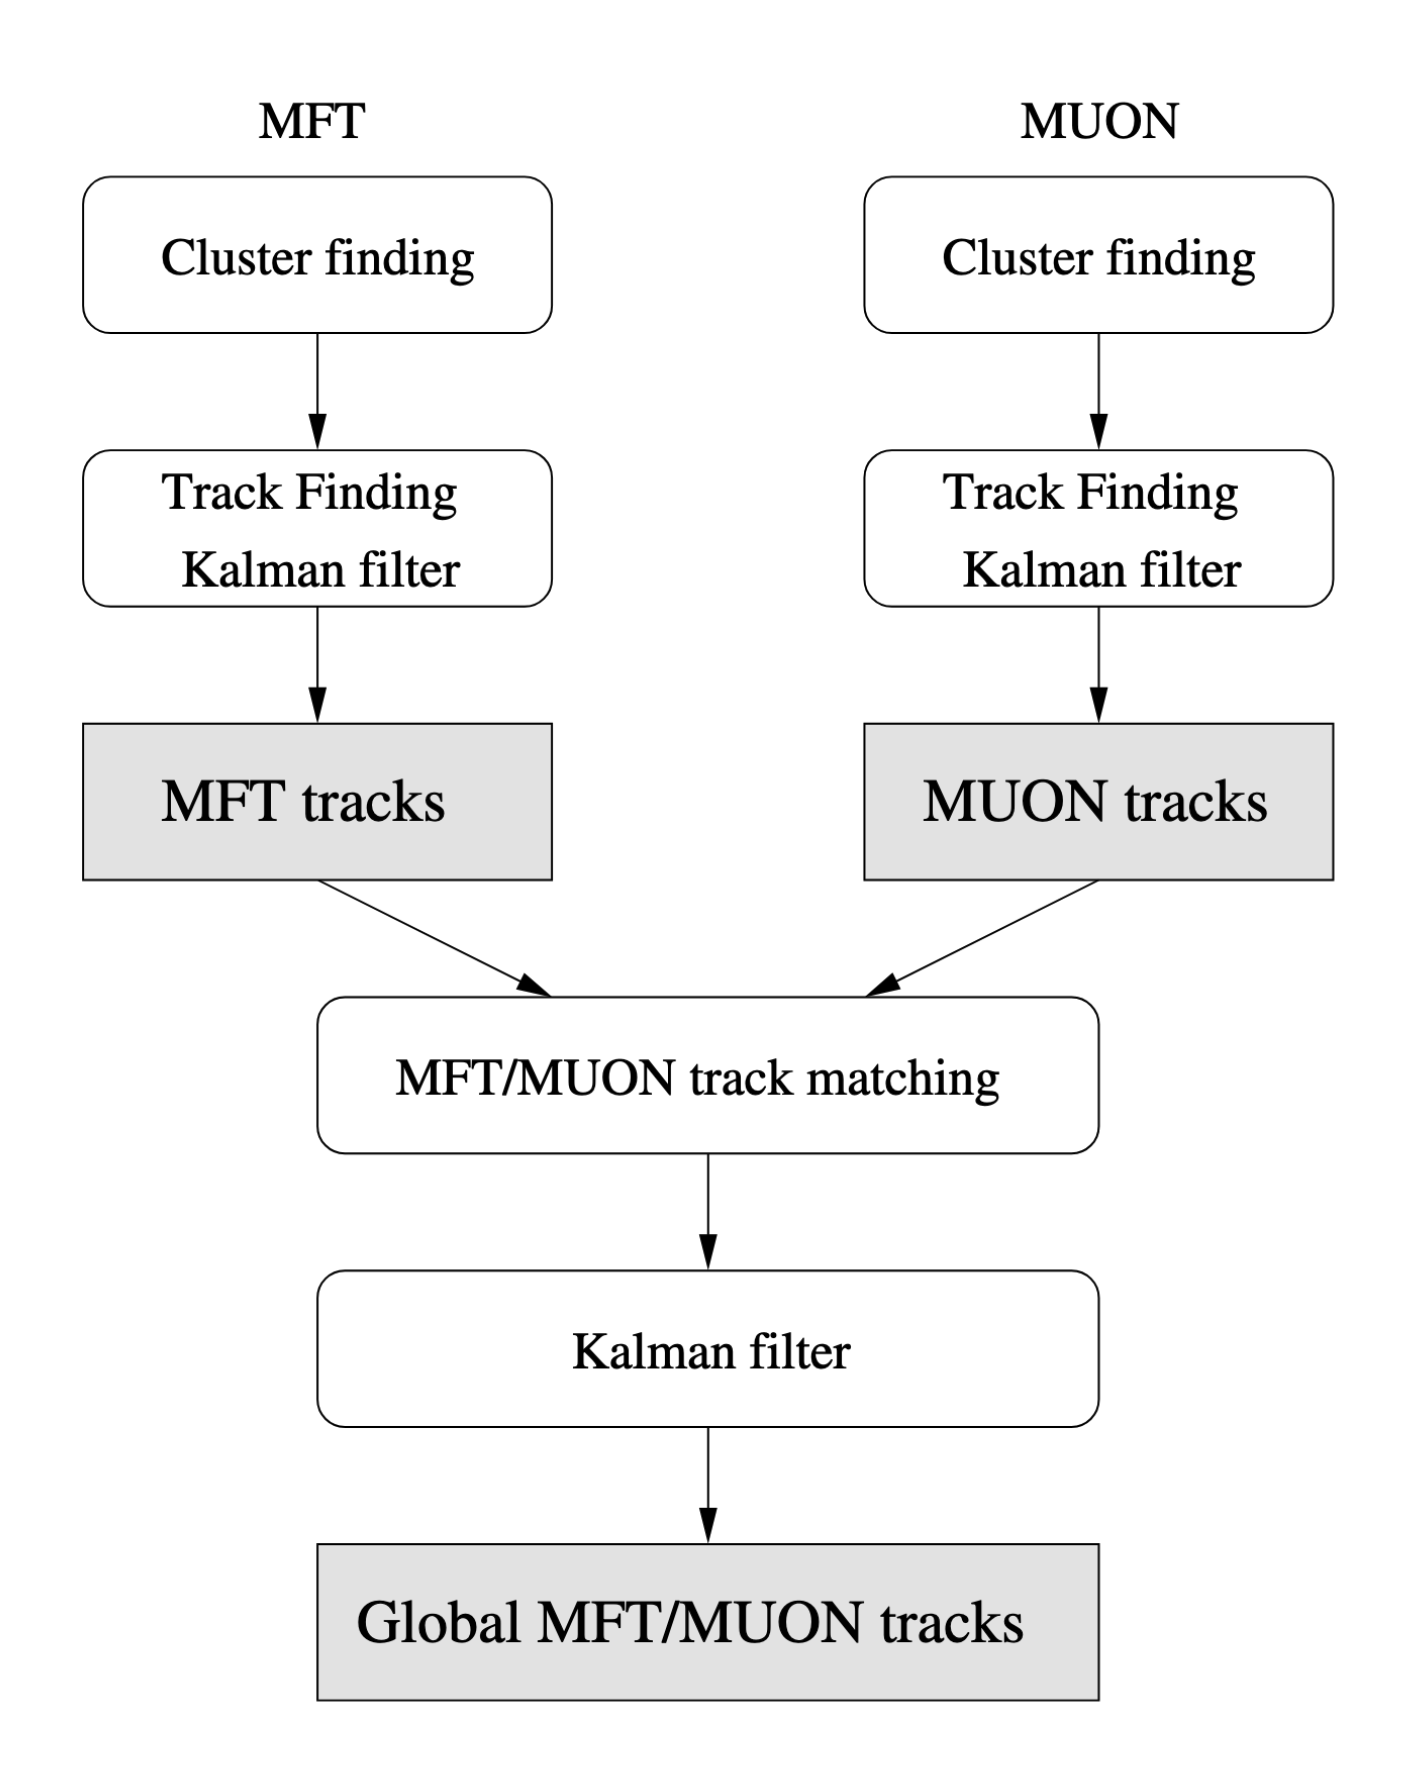
\includegraphics[keepaspectratio, scale=0.3]{fig/2_2_3_GlobalTrackReco.png}
            %    \caption{Global Track\cite{MFT_TDR}}
             %   \label{GlobalTrackReco}
            %\end{figure}
            %MUON spectrometerで測定したMCH TrackとMFTでで測定したMFT Trackを用いてGlobal Trackを再構成した。